\documentclass{beamer}
\usepackage[utf8]{inputenc}
\usepackage{graphicx}
\usepackage{multicol}
\usepackage{soul} % strikethrough
\graphicspath{ {./imgs/} }


\usetheme{metropolis}
\usecolortheme{seahorse}
\setbeamertemplate{frame numbering}[fraction]
\metroset{block=fill}


\title{We Have Built Nice Things}
\subtitle{structured nvim plugins}
\author{Wang, Hao}
\institute{Lead Engineer @ Graveflex | ms-jpq @ github | hola@bigly.dog}
\date{}


\begin{document}


\begin{frame}

	% LaTex tutorial
	% https://www.youtube.com/watch?v=0fsWGg81RwU

	\titlepage

\end{frame}


\begin{frame}{Inspiration}

	We can have nice things - \textit{Justin M. Keyes}

	\vspace{1em}

	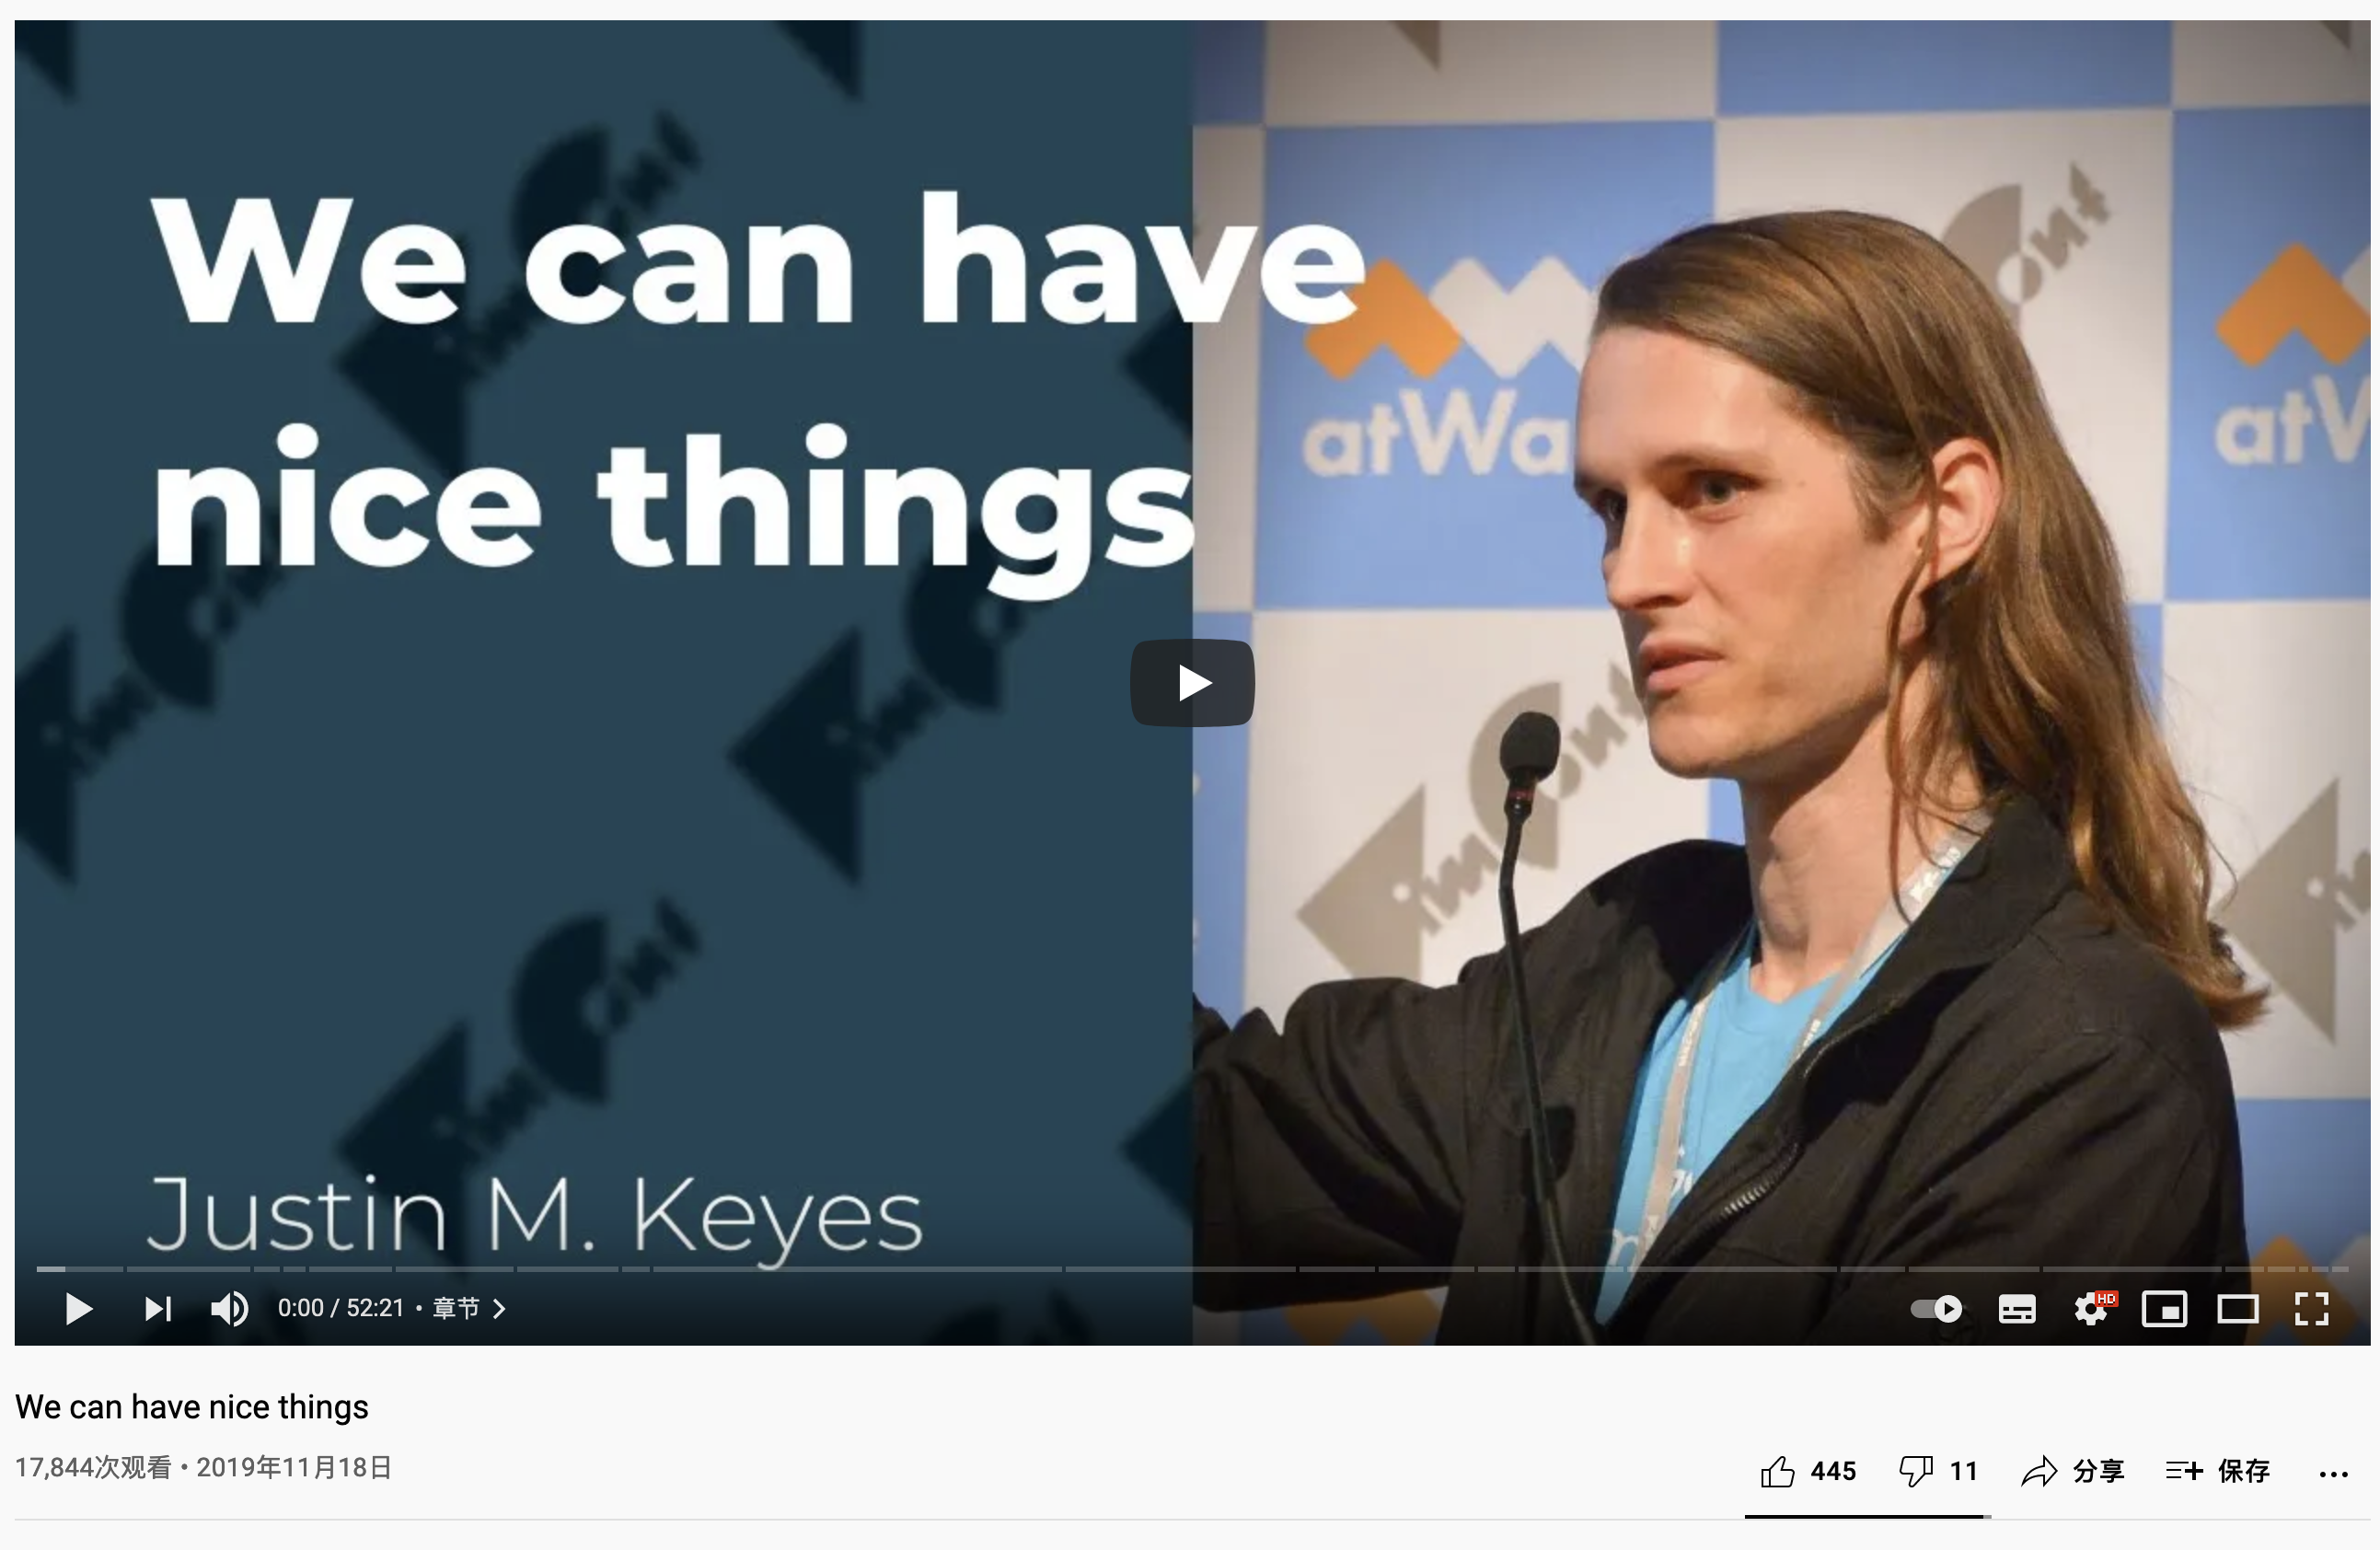
\includegraphics[width=\textwidth]{we_can_have_nice}

\end{frame}


\begin{frame}{Why Nvim?}

	I wanted to replace emacs

	\vspace{1em}

	
\includegraphics[width=\textwidth]{home_page}

	\vspace{1em}

	...and make CLI as easy as VSCode

\end{frame}


\begin{frame}{Vim "philosophy"}

	\begin{itemize}

		\begin{multicols}{2}

			\item unix-y

			\item ad hoc

			\item macro driven

			\item minimalist

			\item extensible

			\item composible

			\item conservative

		\end{multicols}

	\end{itemize}

	\rule{\textwidth}{0.1em}

	\textbf{But at what cost?}

	\begin{itemize}

		\begin{multicols}{2}

			\item slowiness

			\item jankiness

			\item ossification

			\item interlocking

			\item beginner hostile

			\item dx hostile

		\end{multicols}

	\end{itemize}


\end{frame}


\begin{frame}{Terraforming Nvim}
	
	\begin{block}{Terraforming}

		\vspace{0.5em}

		Making nvim more hospitable for developers

		\vspace{0.5em}

	\end{block}

	\rule{\textwidth}{0.1em}

	\begin{itemize}

		\begin{multicols}{2}

			\item lua
			
			\item vim.api.nvim\_*

			\item API clients

			\item tree-sitter

			\item libuv

			\item extmarks

			\item virtual text

			\item remote UI

		\end{multicols}

	\end{itemize}

	... and more 

\end{frame}


\begin{frame}{Tolerance for Heresy}

	Beyond just the API, but also the \textbf{culture too}

	\rule{\textwidth}{0.1em}

	\textbf{Wait, you can do that??}

	\begin{enumerate}

		\item nvim = OS for TUI

		\item buffers = render targets

		\item architecture <- react + redux, data driven

		\item "AOT compiled, statically linked"

		\item Well defined protocols

	\end{enumerate}

\end{frame}


\begin{frame}{Yes We Can}

	Short detour

	\rule{\textwidth}{0.1em}

	Lua is awesome

	You can write \textit{async await} as a \textbf{library}, (first class coroutines)

	https://github.com/ms-jpq/lua-async-await

\end{frame}

% \begin{frame}{What Programmers Like}

% 	\textbf{Structure \& Regularity}

% 	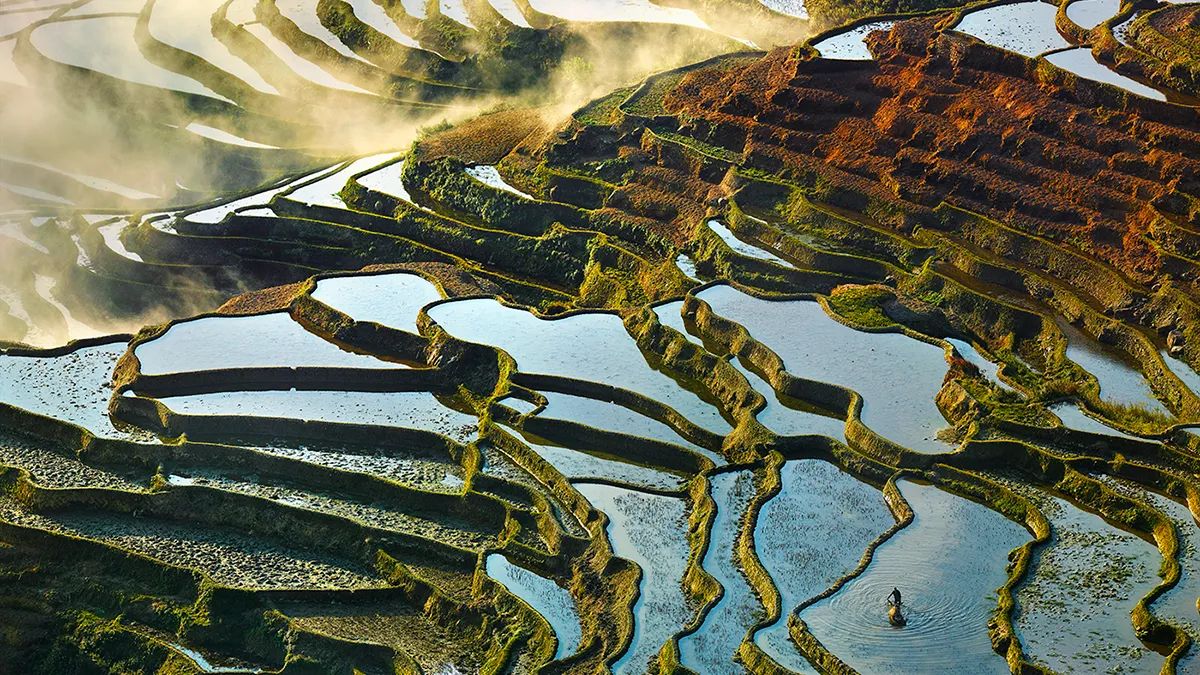
\includegraphics[width=\textwidth]{rice_paddy}

% 	\textit{thousand year old rice paddy}

% \end{frame}


\begin{frame}{AOT Static Linking}

	\begin{block}{\st{Extensibility} Kitchen sink}

		\vspace{0.5em}

		Do one \st{thing} \textbf{domain} and do it well.

		\vspace{0.5em}

	\end{block}

	Bake related features into single plugin

	\rule{\textwidth}{0.1em}

	Still "composible"

	\begin{itemize}

		\item pre-compile third party themes into json

		\item pre-compile third party snippets into json

		\item pre-compile ... into json

	\end{itemize}

\end{frame}


\begin{frame}{CHADTree}

	https://github.com/ms-jpq/chadtree

	\rule{\textwidth}{0.1em}

	\begin{itemize}

		\begin{multicols}{2}
  	
			\item visual multi selection

			\item persistent selection across copy / move

			\item quickfix highlight

			\item glob filtering

			\item trash bin

			\item open with sys

			\item ls -l

			\item follow mode

			\item version control status

			\item \$LS\_COLOUR theming

			\item icons out of box

			\item github derived language colouring

			\item session support

			\item typed config parser
  	
		\end{multicols}

	\end{itemize}

\end{frame}


\begin{frame}{Faster than LUA}

	\begin{block}{Observations}

		\begin{enumerate}

			\item File system walking is very fast

			\item Rendering is slow

			\item Filemanager plugins cause dramatic slowdowns

		\end{enumerate}

	\end{block}

	\begin{block}{Solution}

		\begin{itemize}

			\item Pull in plugin functionalities

			\item Minimize rendering

		\end{itemize}
 	
	\end{block}

	Big tradeoff: lose extensibility

	Big win: no ossification

\end{frame}


\begin{frame}{React Redux}

	I wrote a \textbf{70 line} React before, it's not hard:

	https://github.com/ms-jpq/noact

	\rule{\textwidth}{0.1em}

	Virtual rendering target (store desired state)

	\begin{enumerate}

		\item Compute designed state

		\item Compute linewise hash of desired state

	\end{enumerate}

	Actual rendering target (apply state to buffers)

	\begin{enumerate}

		\item Fetch hash -> compute minimal diff

		\item Apply patch onto buffers, store hash

	\end{enumerate}

\end{frame}


\begin{frame}{COQ.nvim}

	Fast AF auto completion

	https://github.com/ms-jpq/coq_nvim
	
	\begin{block}{Observations}

		\begin{itemize}

			\item Computers are \textit{fast}, humans are \textit{slow}

			\item Typos happen frequently

			\item Completion menu is ad hoc doc viewer

		\end{itemize}
 	
	\end{block}

	\rule{\textwidth}{0.1em}

	Design goals

	\begin{itemize}

		\item High quality ranking

		\item Fuzzy algorithms

		\item As much information as possible

	\end{itemize}

\end{frame}


\begin{frame}{Going in the opposite direction}

	Need to support third party plugins, but...

	Notice a pattern here:

	\begin{enumerate}

		\item nvim-completion-manager -> ncm2

		\item neocomplete.vim -> deoplete.nvim -> ddc.vim

		\item nvim-compe -> nvim-cmp

		\item completion-nvim :: still ok!

		\item YouCompleteMe :: still ok!

		\item coc :: going great!

	\end{enumerate}


\end{frame}


\begin{frame}{The protocols of Nvim}

	Protocols are meant to be ossified

	Implementations are not

	Some protocols inherent to Nvim

	\begin{enumerate}

		\item vim.bo.omnifunc

		\item :h complete-items

		\item vim.lsp.protocol

	\end{enumerate}

\end{frame}


\begin{frame}[standout]

	Q \& A

\end{frame}


\end{document}
